\subsection{EPS}
EPSはClyde Space社の3rd Generation 3U EPSを購入した.
EPSの電気・構造的特性を表\ref{table3_1_eps_spec}に,絶対最大定格を表\ref{table3_1_eps_max}に示す.
\begin{figure}[htbp]
	\begin{center}
		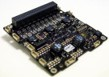
\includegraphics[width=0.5\linewidth]{./03/fig/eps.jpg}
		\caption{EPS}
		\label{eps}
	\end{center}
\end{figure}


\begin{table}[htbp]
	\centering
	\caption{Electrical and Physical Characteristics of EPS \cite{eps_um}}
	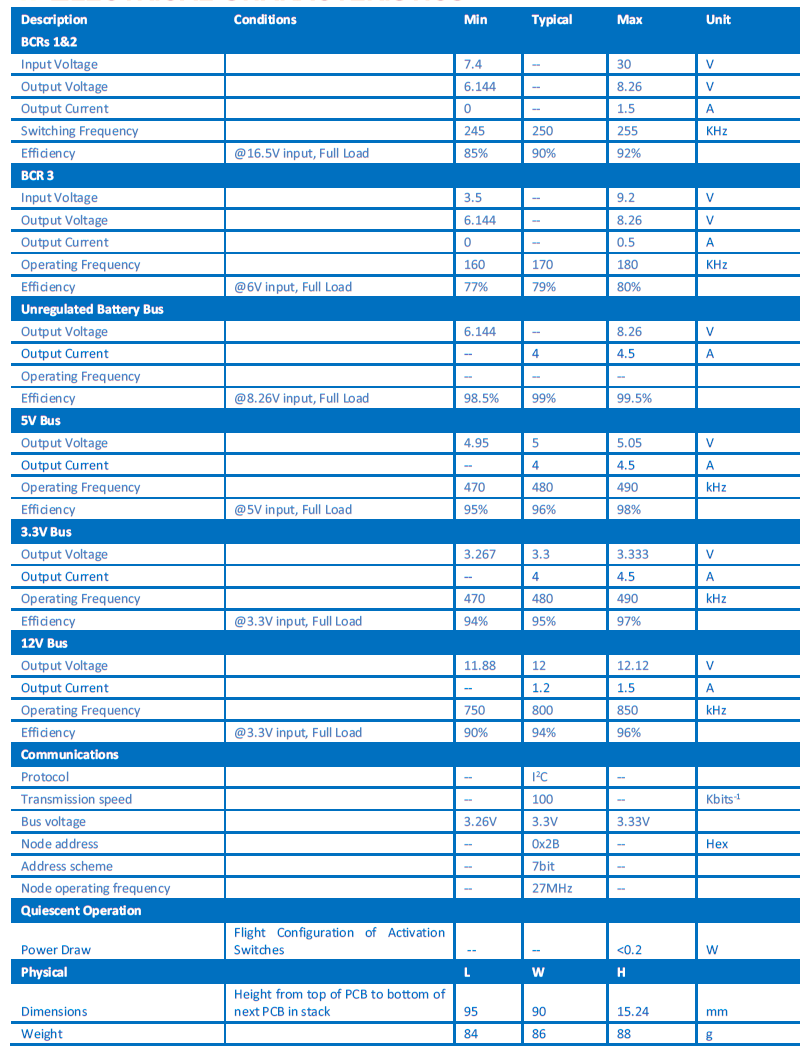
\includegraphics[width=0.9\linewidth]{./03/fig/eps_spec.png}
	\label{table3_1_eps_spec}
\end{table}

\begin{table}[htbp]
	\centering
	\caption{Maximum Ratings of EPS \cite{eps_um}}
	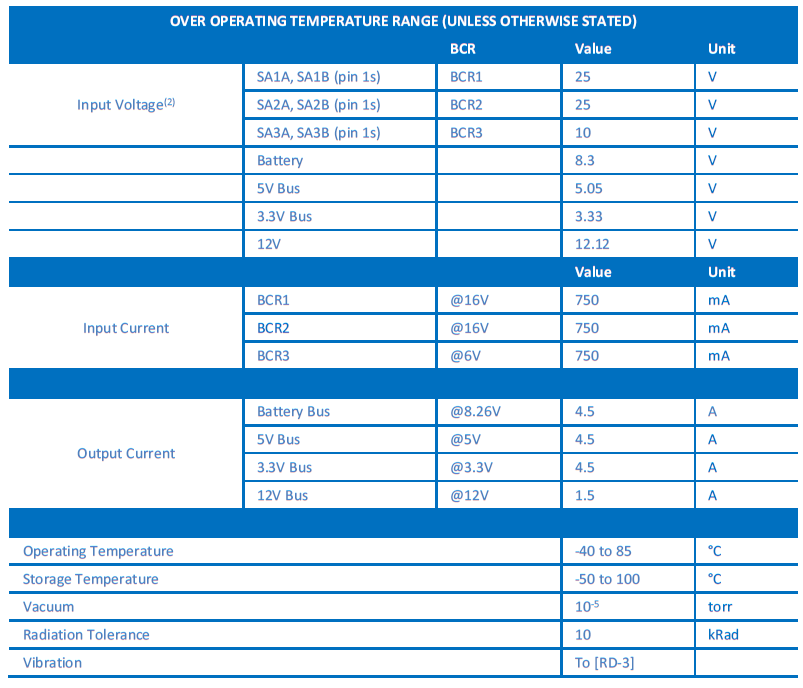
\includegraphics[width=0.9\linewidth]{./03/fig/eps_max.png}
	\label{table3_1_eps_max}
\end{table}


EPSユーザーマニュアル記載のEPSおよびSAP,Batteryを含めた機能図を図\ref{fig3-1_eps_bd}に示す.なお本衛星ではBattery-EPS間,SAP-EPS間にインヒビット回路が組み込まれているため実際のコンフィグレーションとは異なる.EPSの各スイッチのON/OFFはOBCからの$\mathrm{I^{2}C}$によって制御された.

\begin{landscape}
\begin{figure}[H]
	\centering
	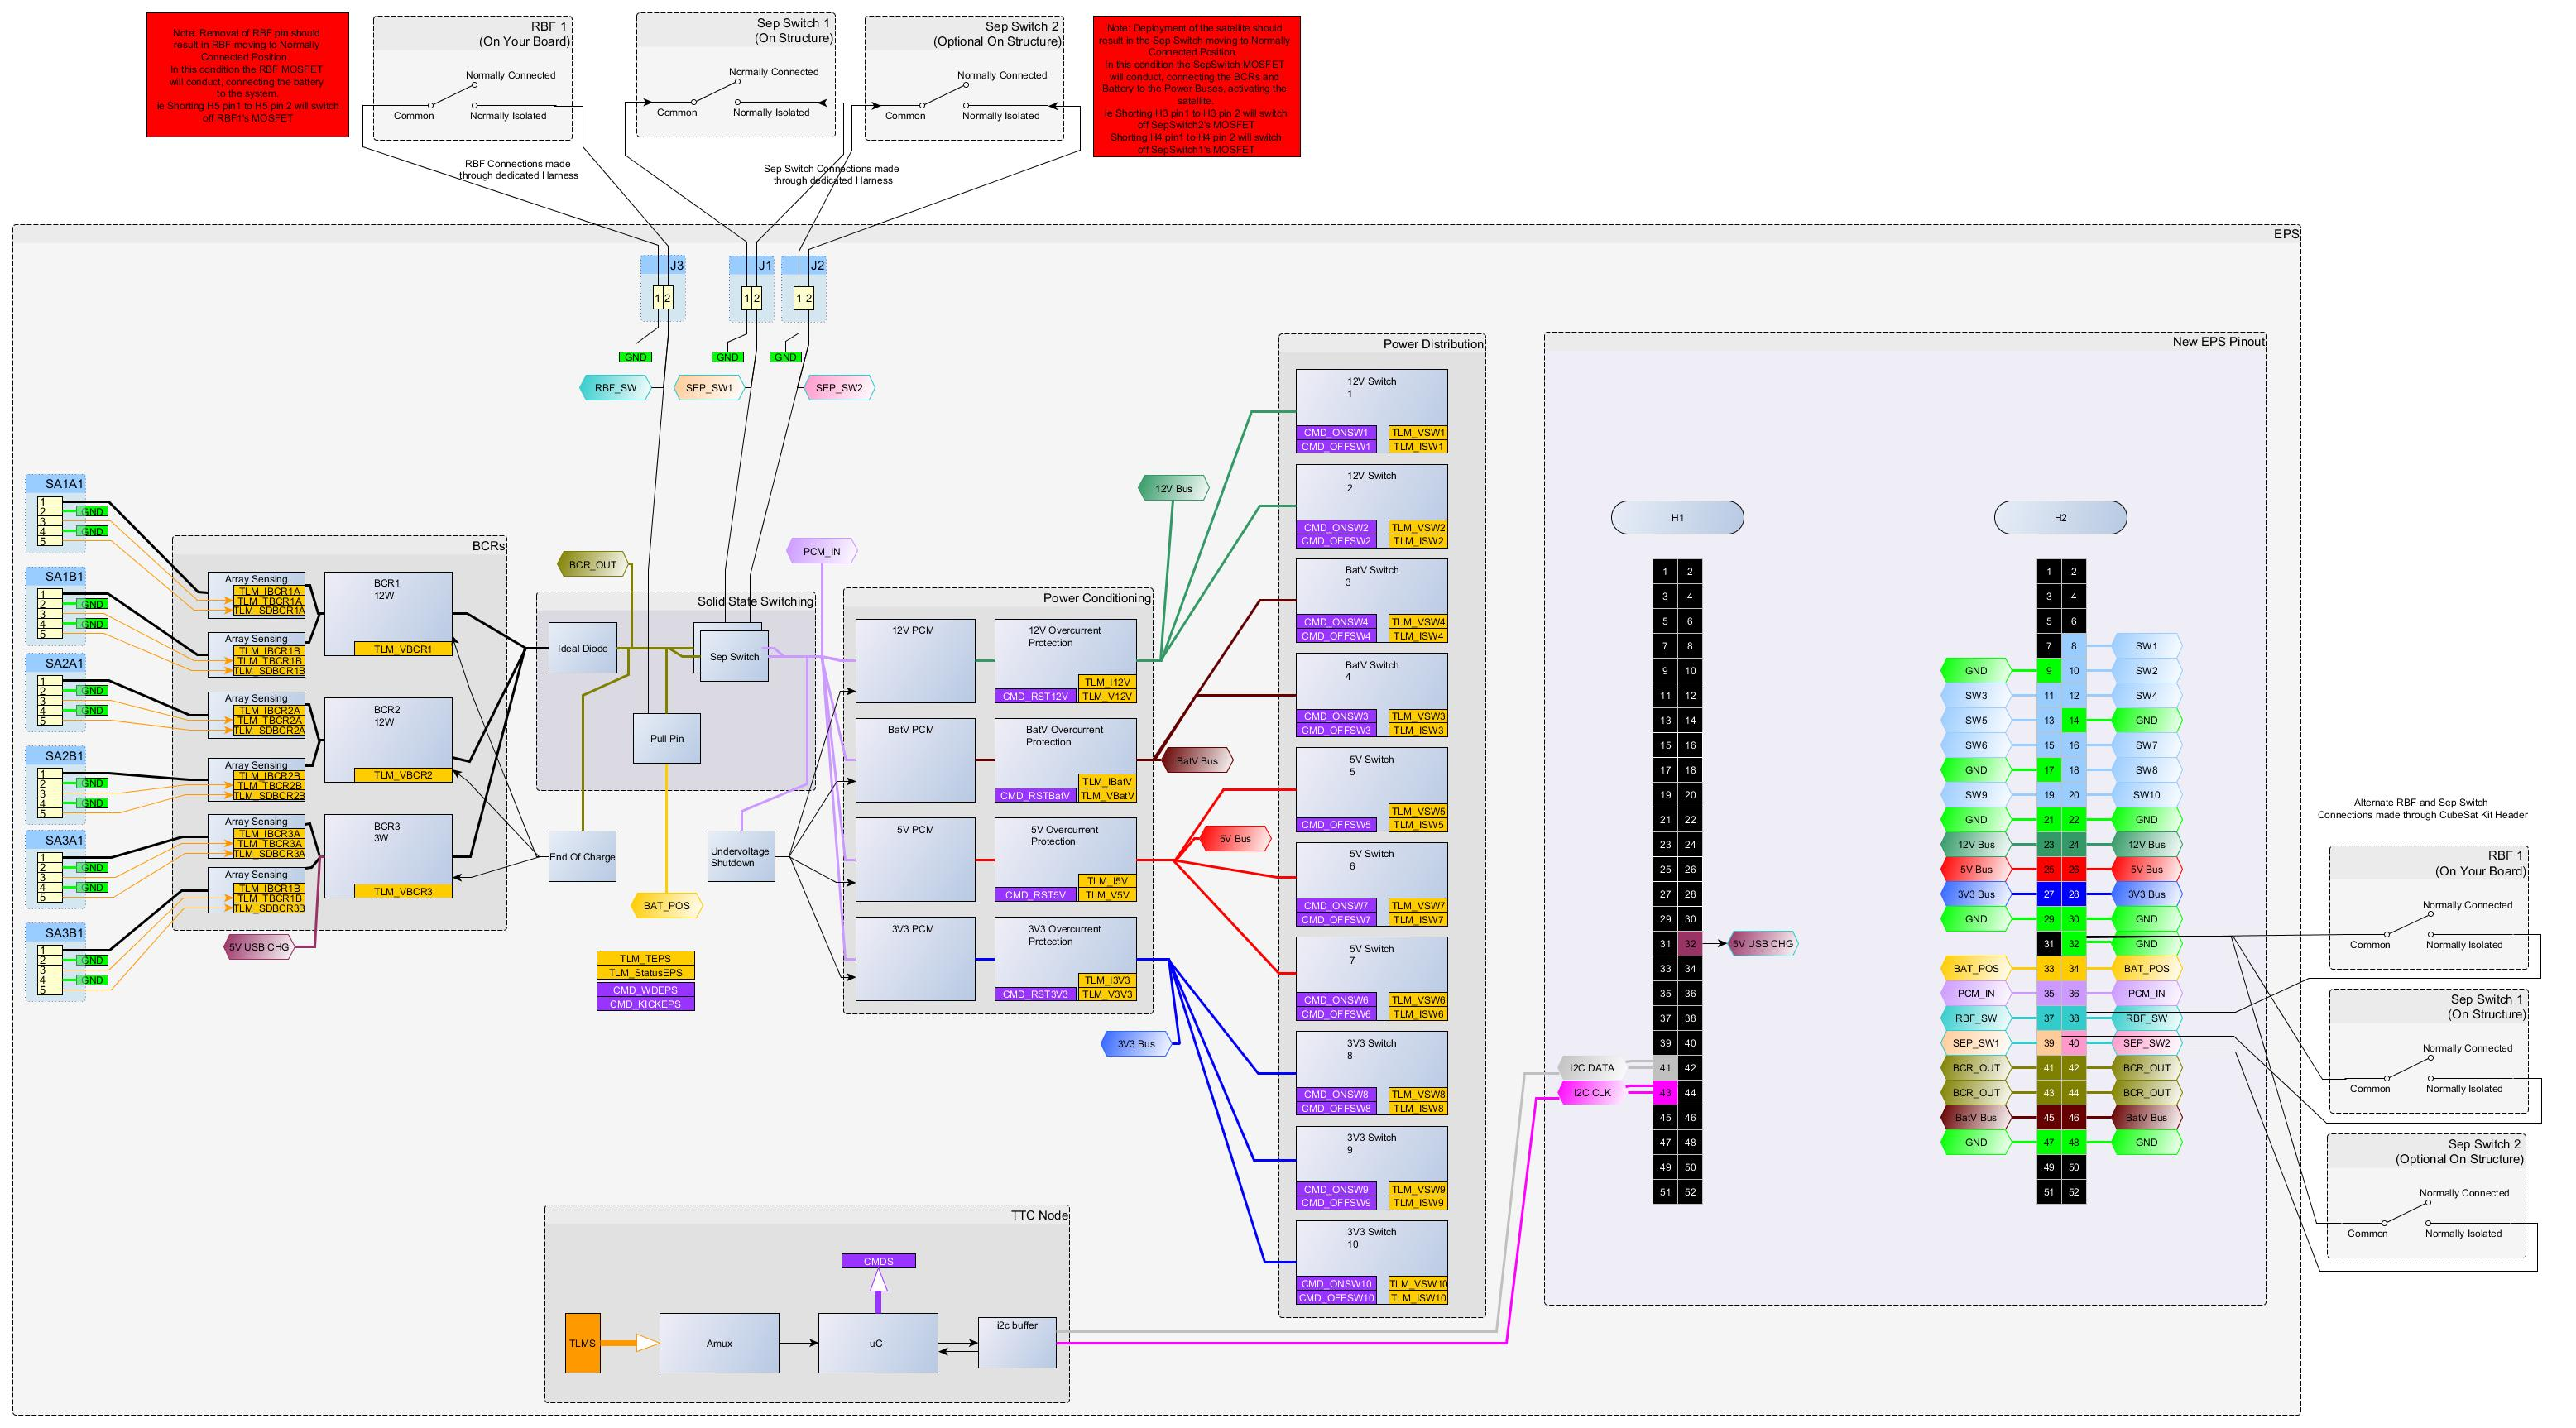
\includegraphics[width=0.9\linewidth]{./03/fig/eps_bd.jpg}
	\caption{Functional Diagram of EPS \cite{eps_um}}
	\label{fig3-1_eps_bd}
\end{figure}
\end{landscape}